\documentclass{article}
\usepackage[utf8]{inputenc}

% Code packages and configurations
\usepackage{color}
\usepackage{float}
\usepackage{graphicx}
\usepackage{listings}
\usepackage{url}

\definecolor{dkgreen}{rgb}{0,0.6,0}
\definecolor{gray}{rgb}{0.5,0.5,0.5}
\definecolor{mauve}{rgb}{0.58,0,0.82}

\lstset{frame=tb,
  language=Java,
  aboveskip=3mm,
  belowskip=3mm,
  showstringspaces=false,
  columns=flexible,
  basicstyle={\small\ttfamily},
  numbers=none,
  numberstyle=\tiny\color{gray},
  keywordstyle=\color{blue},
  commentstyle=\color{dkgreen},
  stringstyle=\color{mauve},
  breaklines=true,
  breakatwhitespace=true,
  tabsize=3
}

\title{People Identification}
\author{David Suárez}
\date{\today}

\begin{document}

\maketitle

\section{Introducción}
Este documento describe tanto el proceso de desarrollo como el proceso de investigación previo para poder realizar un proyecto basado en una tecnología innovadora como es Tensorflow junto con diferentes técnicas aplicadas para obtener el resultado más eficiente.
Tras un proceso previo de investigación que a continuación explicaré, el proyecto finalmente podría dividirse en tres partes claramente diferenciadas.
\begin{itemize}
\item Identificación de personas utilizando redes neuronales multicapa.
\item Identificación de personas utilizando redes neuronales convolucionales.
\item Procesamiento en streaming de imágenes utilizando la red neuronal.
\end{itemize}

\section{Objetivo}
El objetivo de este proyecto es el reconocimiento e identificación de personas concretas básandonos en su rostro. Para ello hemos hecho un proceso de investigación que explicaremos a continuación y que ha estado dividio en diferentes fases finalizando con una conclusión en la que se explican los diferentes resultados obtenidos.

\section{Fases de investigación y desarrollo}
Distinguimos diferentes fases de investigación y desarrollo.\newline

Con respecto a la parte de investigación podemos diferenciar las siguientes:
\begin{itemize}
\item Resolución de problemas relativo a la identificación de una cara en una imagen
\item Diferentes métodos para obtener información de la cara relativa a la posición de los ojos, la boca, etc.
\item Diferentes algoritmos posibles para la obtención del mayor porcentaje de acierto realizando una predicción.
\end{itemize}

Con respecto a la parte de desarrollo podemos diferenciar las siguientes:
\begin{itemize}
\item Procesado de imágenes con diferentes librerías como dlib, Haar Cascades para identificación de caras y puntos de referencia.
\item Entrenamiento y modelado de redes neuronales utilizando Tensorflow.
\item Creación de un flujo de imágenes en streaming que haga uso del modelo entrenado para dar una predicción.
\end{itemize}

\section{Identificacion de caras}
En este punto nos referimos al estudio y procesado de imágenes para la identificacion de caras en ella, es decir, no queremos identificar a la persona aun, simplemente distinguir entre la cara y el resto del cuerpo.

La solución a este problema está ya bastante optimizada, existen varias librerías en el mercado que lo solventan. Primero ha sido testeado mediante el uso de openCV, utilizando haar cascades cuyos resultados fueron buenos y posteriormente he terminado utilizando Dlib, ya que tiene un método creado específicamente para ello y los resultados eran mejores.

\begin{figure}[H]
  \centering
  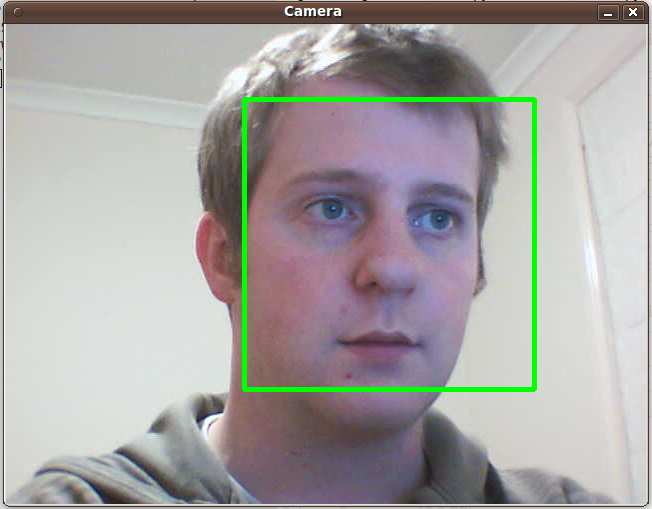
\includegraphics[width=100mm, height=80mm]{images/face-detect_square.png}
  \caption{Imagen 1}
\end{figure}

\section{Landmarks}
Para este problema hemos probado dos soluciones diferentes, ambas basadas en openCV.  

\subsection{Haar Cascades}
La primera ha sido utilizando haar cascades de los ojos y la sonrisa, lo cual no daba un resultado muy óptimo ya que a veces no era capaz de detectar ambos ojos, o no era capaz de detectar la boca, es decir, la salida de este algoritmo era un vestor cuyo tamaño era variable dependiendo de lo que detectaba. Esto causaba muchos problemas a la hora de introducir los datos en la red neuronal ya que el número de entradas no puede variar. En el caso de streaming esto era especialmente problemático ya que era más dificultoso filtrar los frames que no habían sido correctamente clasificados por lo que esta opción fue desechada.

\begin{figure}[H]
  \centering
  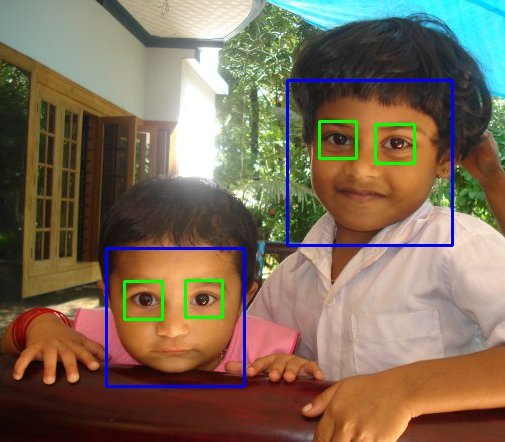
\includegraphics[width=100mm, height=80mm]{images/face_detection_haar_cascades.jpg}
  \caption{Detección de cara y ojos haar cascades}
\end{figure}

\subsection{Dlib}
Esta ha sido mi segunda opción y la definitiva debido a su efectividad. El algoritmo nos devuelve 68 puntos(landmarks) que pueden verse en la imagen inferior y que posteriormente procesamos mediante nuestro algoritmo de cálculo de distancias que explicaré a continuación.
 
\begin{figure}[H]
  \centering
  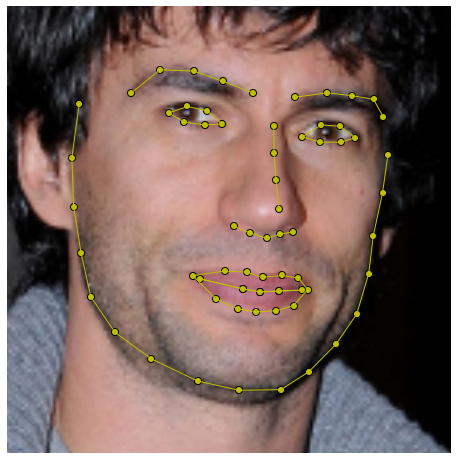
\includegraphics[width=100mm, height=80mm]{images/landmarked_image.png}
  \caption{Detección de landmarks Dlib}
\end{figure}

\section{Algoritmo de cálculo de distancias}
Para nuestra primera rama de investigación en la que utilizaremos una red neuronal multicapa he diseñado un algoritmo que calcula distancias entre diferentes puntos de la cara(landmarks) creando una matriz de entrada a la red multicapa basada en estas mediciones. A continuación figuran varias imágenes que representan con líneas las mediciones tomadas. Todas estas medidas son posteriormente normalizadas utilizando la distancia total del tabique nasal, para evitar errores en las mediciones en caso de que las fotos sean tomadas desde diferentes distancias con respecto a la cámara.

\begin{figure}[H]
  \centering
  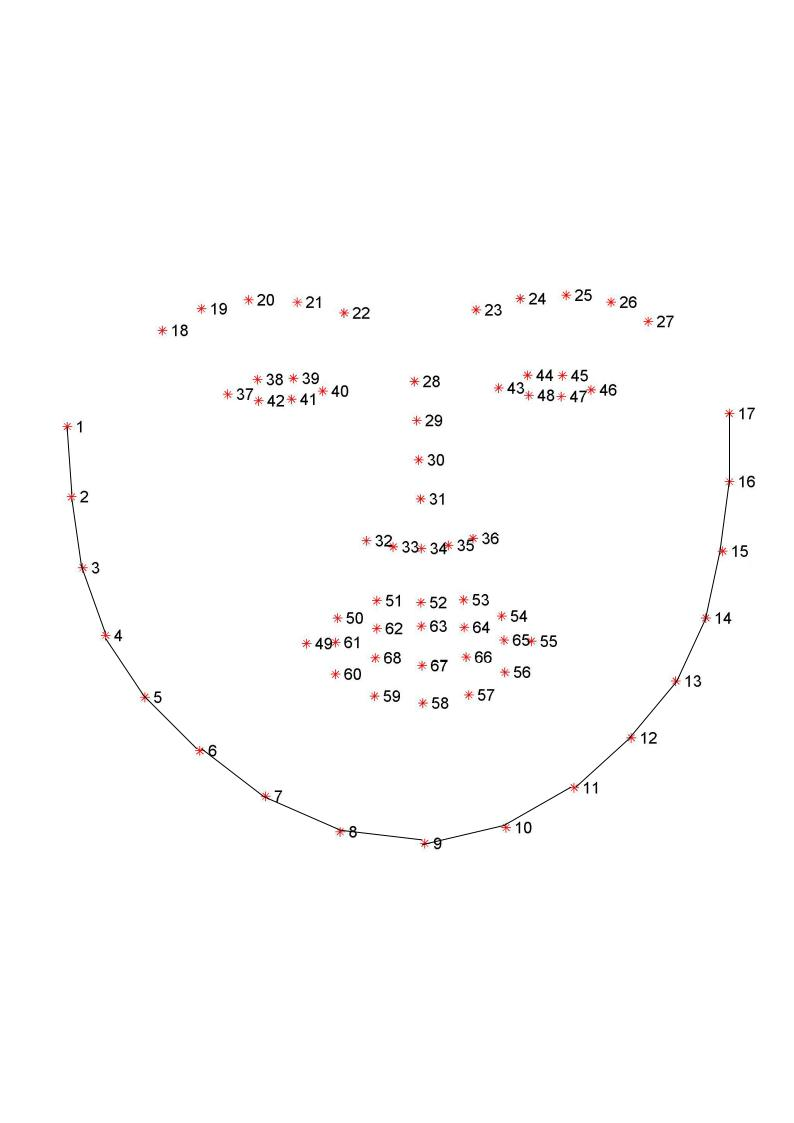
\includegraphics[width=100mm, height=80mm]{images/border_distances.jpg}
  \caption{Perímetro}
\end{figure}


\begin{figure}[H]
  \centering
  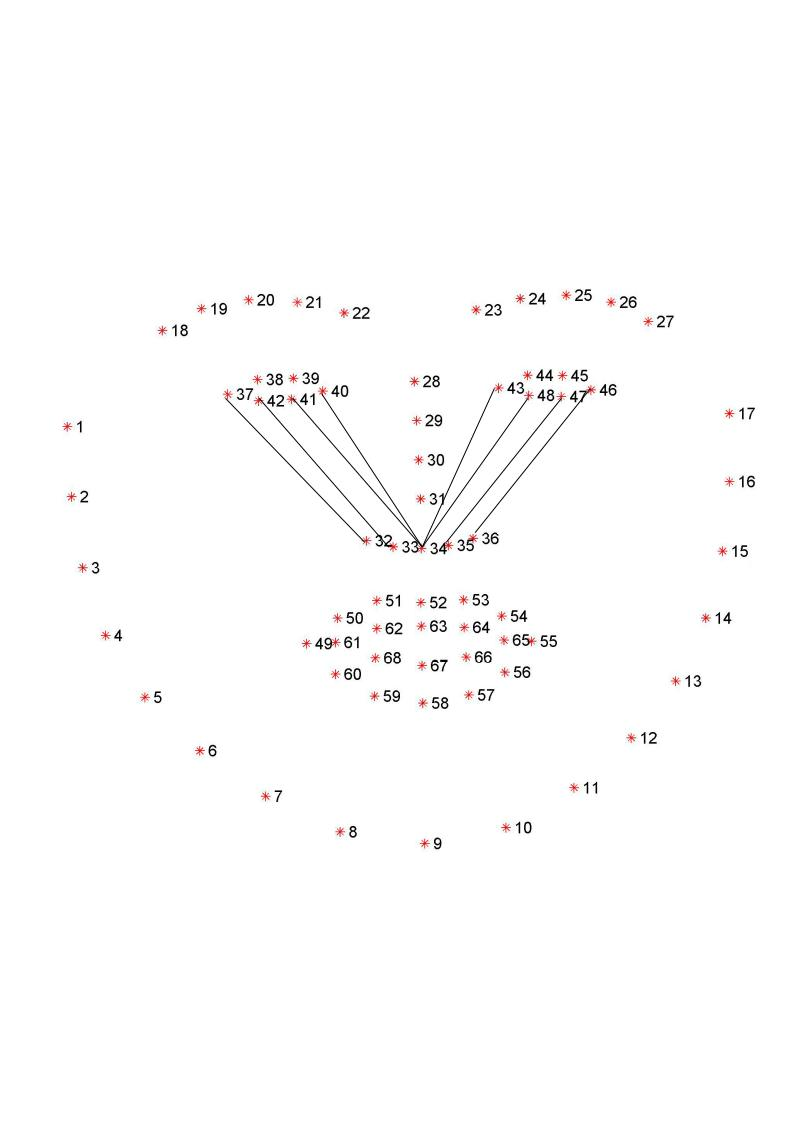
\includegraphics[width=100mm, height=80mm]{images/cheekbone_distances.jpg}
  \caption{Ojos - Naríz}
\end{figure}


\begin{figure}[H]
  \centering
  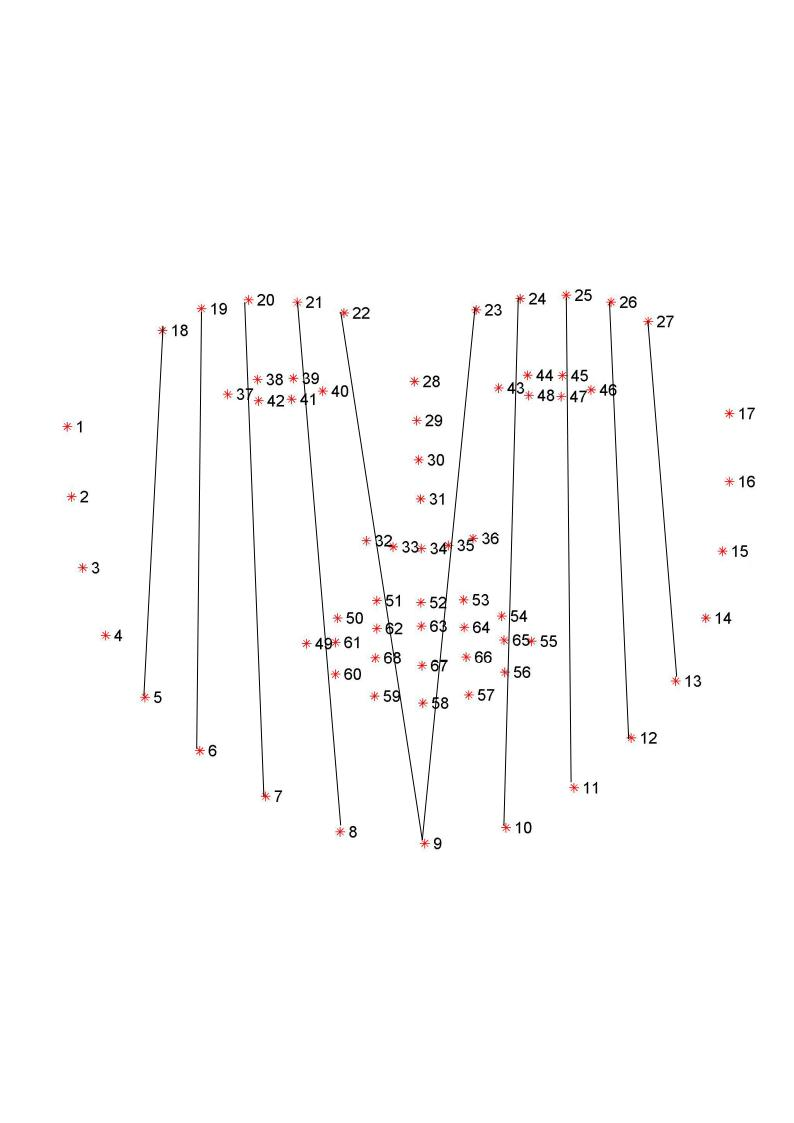
\includegraphics[width=100mm, height=80mm]{images/height_distances.jpg}
  \caption{Cejas - Barbilla}
\end{figure}


\begin{figure}[H]
  \centering
  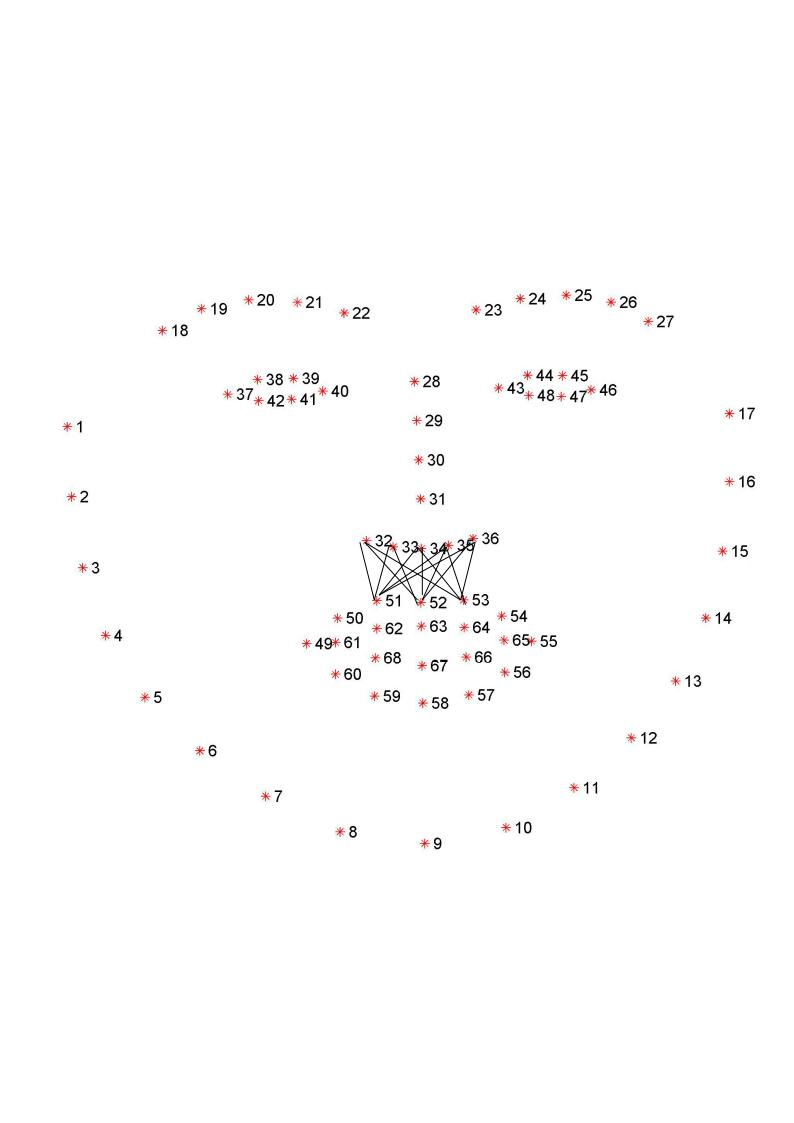
\includegraphics[width=100mm, height=80mm]{images/moustache_distances.jpg}
  \caption{Naríz - Boca}
\end{figure}  
  
\begin{figure}[H]
  \centering
  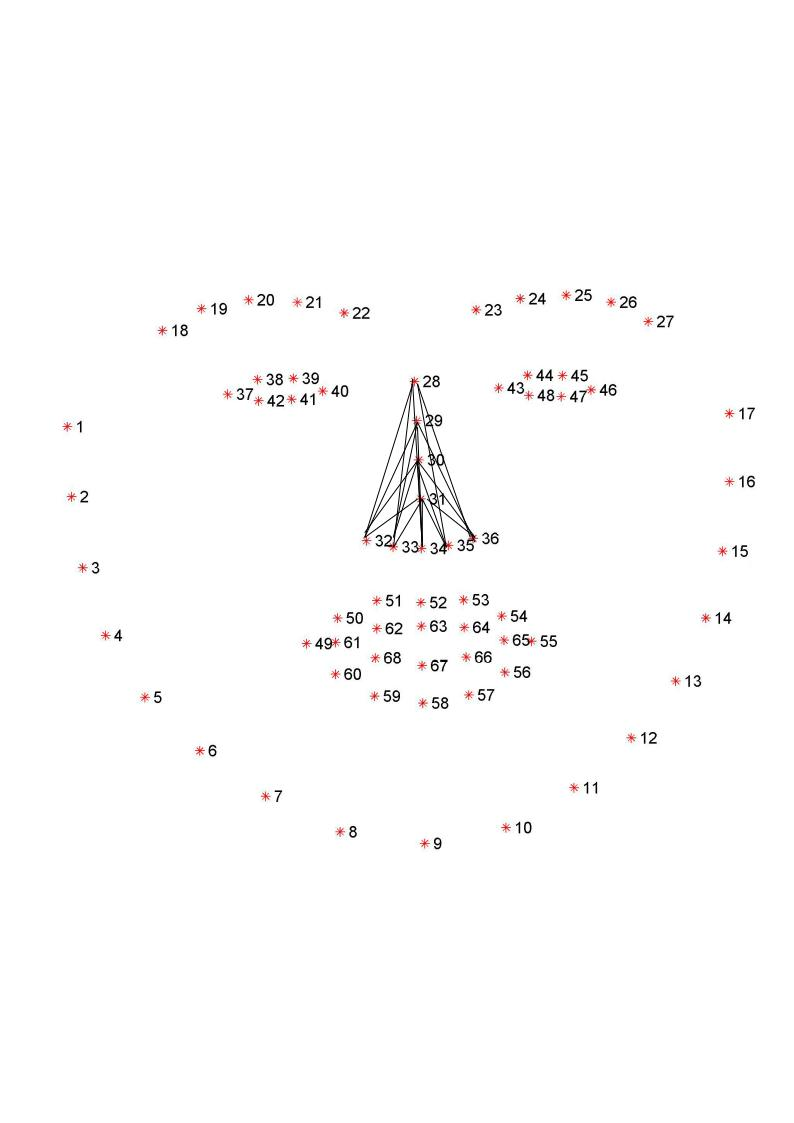
\includegraphics[width=100mm, height=80mm]{images/nasal_septum_distances.jpg}
  \caption{Naríz}
\end{figure}
  
\begin{figure}[H]
  \centering
  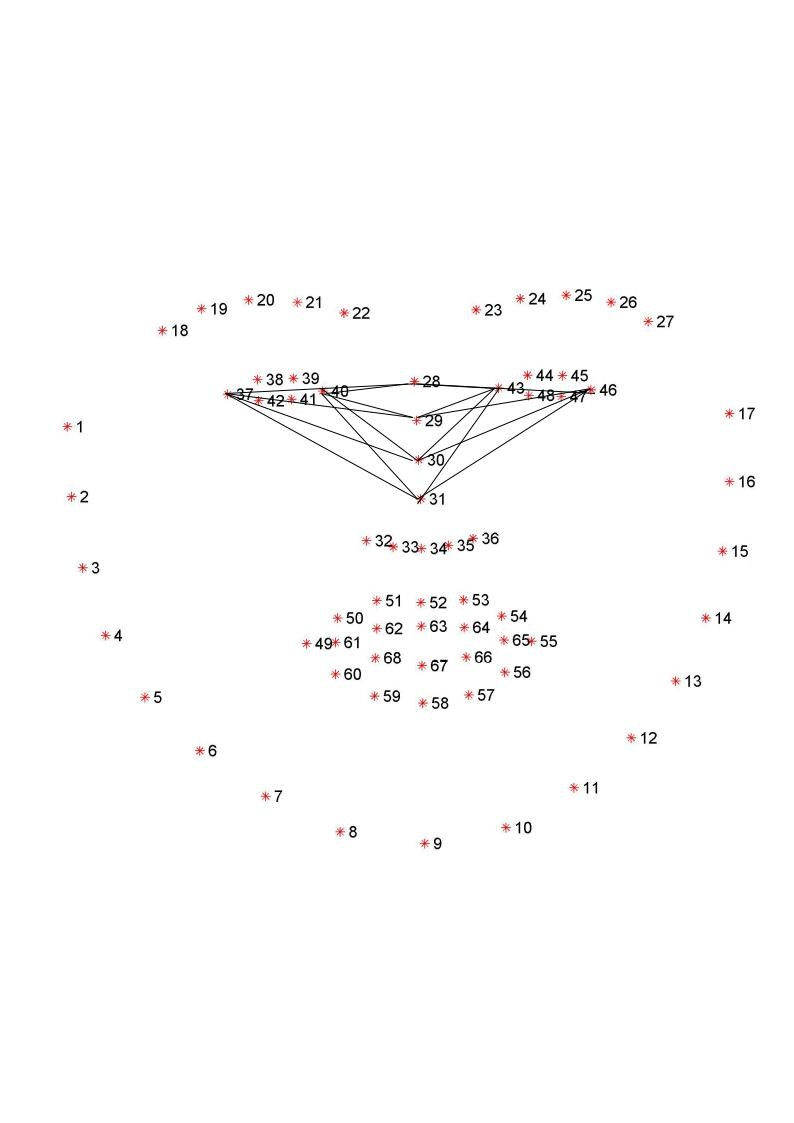
\includegraphics[width=100mm, height=80mm]{images/nose_distances.jpg}
  \caption{Ojos - Naríz}
\end{figure} 
  
\begin{figure}[H]
  \centering
  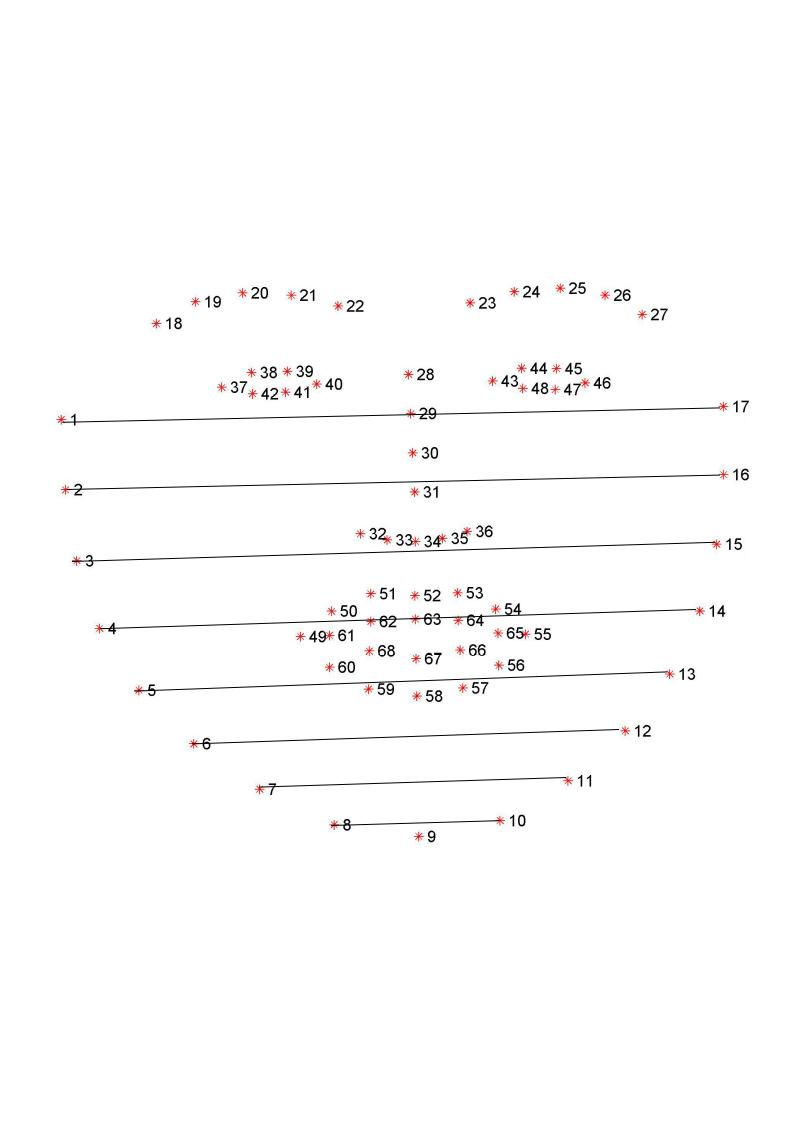
\includegraphics[width=100mm, height=80mm]{images/width_distances.jpg}
  \caption{Ancho}
\end{figure}

\section{Red Neuronal Multicapa}

Para el desarrollo de las redes neuronales como ya he nombrado anteriormente he usado la librería TensorFlow \cite{tensorflow2015-whitepaper}, en concreto su API para Python.

Las Redes Neuronales Artificiales (RNA) \cite{RNA} son sistemas de procesamiento de la información cuya estructura y funcionamiento están inspirados en las redes neuronales biológicas. Consisten en un gran número de elementos simples de procesamiento llamados nodos o neuronas que están organizados en capas(entrada, ocultas y salida). Cada neurona está conectada con otras neuronas mediante enlaces de comunicación, cada uno de los cuales tiene asociado un peso. En los pesos se encuentra el conocimiento que tiene la RNA acerca de un determinado problema.

\begin{figure}[H]
  \centering
  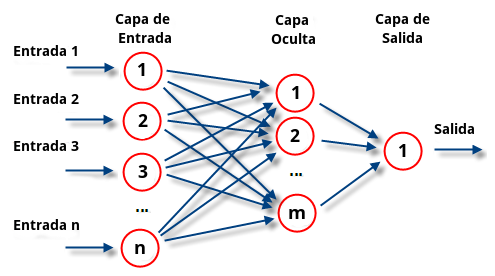
\includegraphics[width=100mm, height=80mm]{images/multilayer_nn.png}
  \caption{Multilayer Representation}
\end{figure}


Entrando un poco más en detalle y ayudándonos del gráfico inferior podemos describir el flujo que sigue una red neuronal. En primer plano tenemos la capa de entrada, que tiene tantas neuronas como longitud tiene nuestro vector de entrada a la red. En segundo plano se sitúa la capa oculta(en este caso solo tenémos una pero puede haber más) la cual es la que contiene la información de la red(los pesos). Estos pesos se van calculando utilizando la función de coste(loss function) \cite{loss_function} la cual nos mide el error de nuestra predicción para que de una manera iterativa nuestra red pueda ir aprendiendo(aprender es encontrar un mínimo de esta función) y de esta manera obtener los pesos óptimos para los cuales el resultado de nuestra predicción sea efectivo.
En la capa de salida se sitúa lo que llamamos la función de activación \cite{activation_function}. Esta función se encarga de definir la salida de la red a partir de los datos que obtenemos de la capa oculta. Un ejemplo de esta sería la función sigmoide \cite{sigmoid} que define la salida de tu red como 0 ó 1.

En nuestro caso hemos utilizado la función softmax \cite{softmax} que es una variante de la sigmoide en la que la salida es un vector de 0s y 1s de tal manera que en caso de que nuestra red quiera diferenciar entre tres personas diferentes la salida siempre será (0, 0, 1) ó (0, 1, 0) ó (1, 0, 0).
\begin{figure}[H]
  \centering
  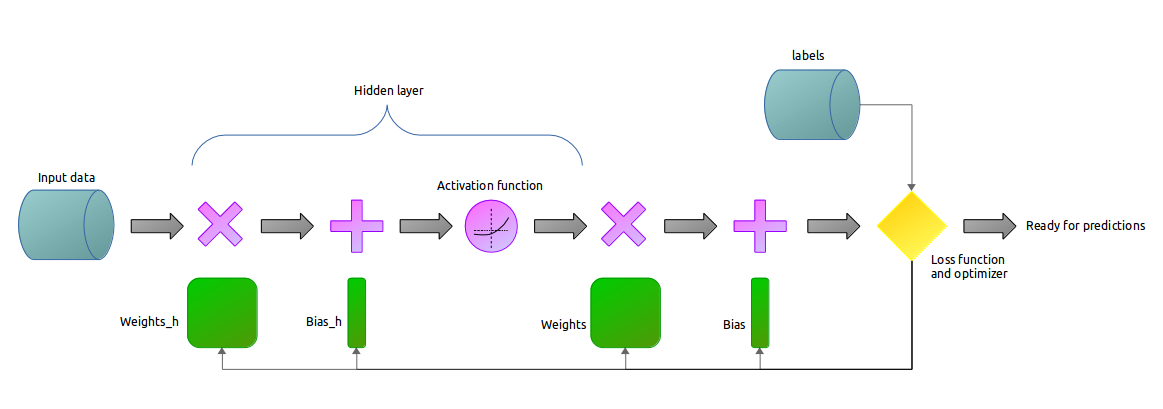
\includegraphics[width=100mm, height=80mm]{images/hidden_nn.png}
  \caption{Multilayer Architecture}
\end{figure}

\begin{figure}[H]
  \centering
  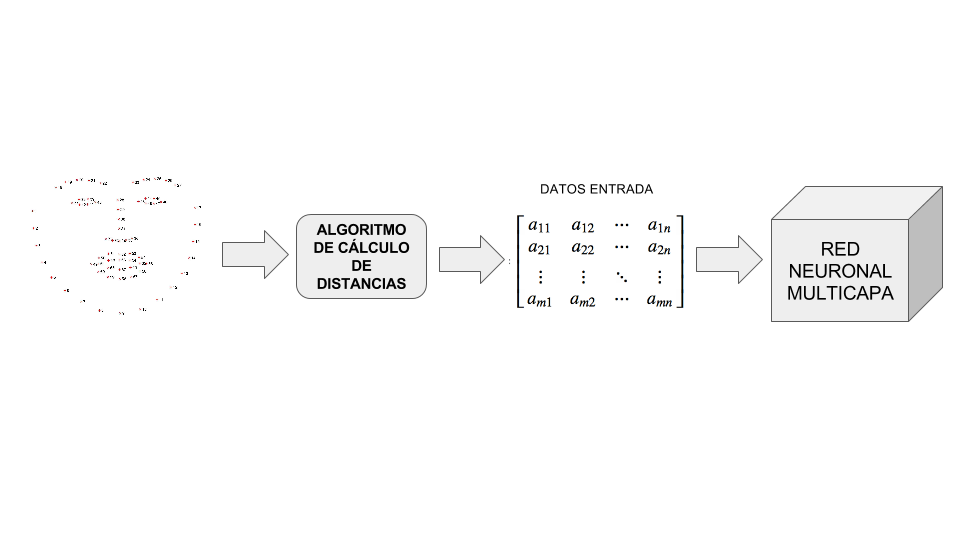
\includegraphics[width=100mm, height=80mm]{images/Flowchart.png}
  \caption{Multilayer Architecture}
\end{figure}


\section{Red Neuronal Convolucional}

A diferencia de la arquitectura anterior la red convolucional usa como datos de entrada imágenes.

La estructura de la red también cambia respecto a la anterior. A modo de resumen, la Red Neurononal Convolucional \cite{RNC} aplica sus transformaciones mediante un \textit{kernel} con el que se van obteniendo los píxeles de la imagen que mejor representan características de nuestros datos. Estas transformaciones se aplican capa a capa, reduciendo el tamaño de la imagen pero aumentando el mapa de características de la misma. Después de todas las transformaciones se obtiene la predicción de los parámetros como en los casos anteriores.

\begin{figure}[H]
  \centering
  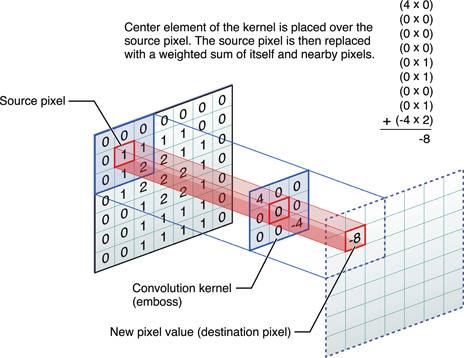
\includegraphics[width=100mm, height=80mm]{images/conv_nn_squema.jpg}
  \caption{Multilayer Architecture}
\end{figure}

Nuestra red consistirá de cuatro capas convolucionales, dos capas ocultas y la capa de salida. A continuación podemos ver un gráfico que explica de manera simple el cálculo de la salida final de la red.

\begin{figure}[H]
  \centering
  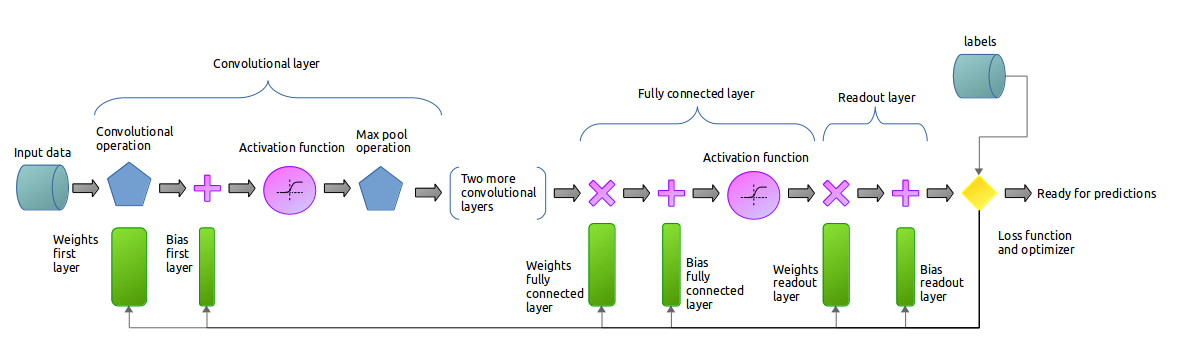
\includegraphics[width=100mm, height=80mm]{images/conv_nn.png}
  \caption{Ancho}
\end{figure}

En el gráfico inferior podemos observar el proceso de aprendizaje de la red mediante la representación de la precisión de la red y la función de coste en relación al número de iteraciones sobre los datos de entrenamiento.

En este primer gráfico podemos ver representadas dos funciones, la primera(verde) es la precisión sobre el conjunto de entrenamiento y la segunda(azul) es la precisión sobre el conjunto de test.

\begin{figure}[H]
  \centering
  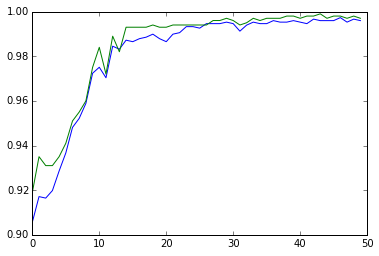
\includegraphics[width=100mm, height=80mm]{images/accuracy.png}
  \caption{Ancho}
\end{figure}

En este siguiente gráfico vemos representada la función de coste, que como podemos observar va disminuyendo el error en la predicción conforme vamos iterando.

\begin{figure}[H]
  \centering
  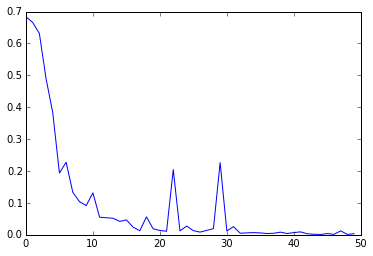
\includegraphics[width=100mm, height=80mm]{images/loss_function.png}
  \caption{Ancho}
\end{figure}

La entrada de la imagen consiste en el recorte de la cara detectada en la imagen como se puede ver de manera descriptiva en el grafico inferior. He realizado diferentes pruebas aplicando filtros a la imagen recortada, como podría ser reducir la imagen a blanco y negro pero los resultados obtenidos no han sido buenos por lo que he decidido dejarla en su estado original.

\begin{figure}[H]
  \centering
  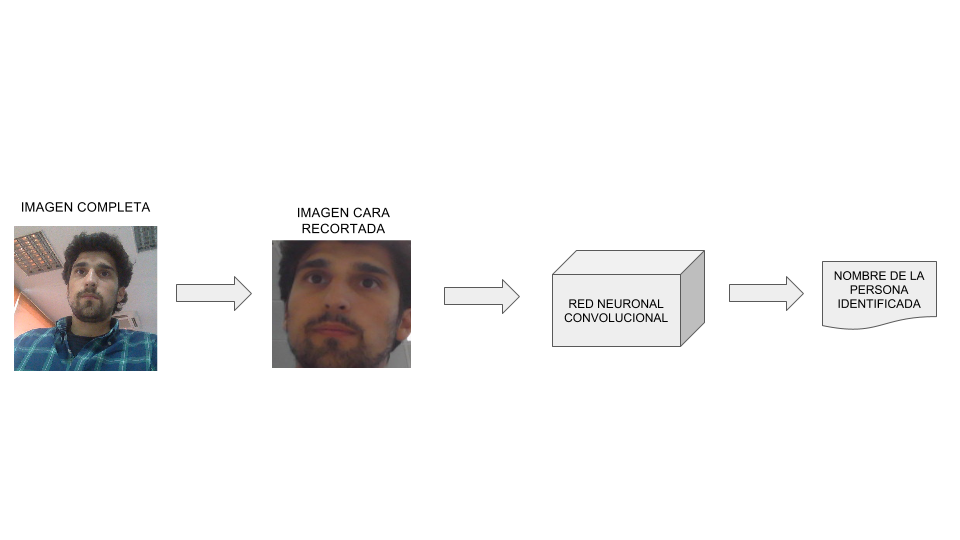
\includegraphics[width=100mm, height=80mm]{images/Flowchart_conv.png}
  \caption{Multilayer Architecture}
\end{figure}

\section{Resultados}
Finalmente y a modo de conclusión procederé a la explicación de los resultados obtenidos mediante ambas ramas de investigación:

\subsection{Red Neuronal Multicapa y Algoritmo de cálculo de distancias}


\subsection{Red Neuronal Convolucional}

\subsection{Demo}
Youtube Link:
https://youtu.be/RxMD2-Wopdw

\bibliographystyle{plain}
\bibliography{turtleflow}

\end{document}